\documentclass{article}

\usepackage{fancyhdr}
\usepackage{extramarks}
\usepackage{amsmath}
\usepackage{amsthm}
\usepackage{amsfonts}
\usepackage{tikz}
\usepackage[plain]{algorithm}
\usepackage{algpseudocode}
\usepackage{graphicx}
\usepackage{gensymb}
\usepackage{calc}
\usepackage[framed,numbered,autolinebreaks,useliterate]{mcode}
\usepackage{listings}
\usepackage{empheq}
\usepackage{enumitem}
\usepackage[font=footnotesize]{caption}

\graphicspath{{./images/}}

\usetikzlibrary{automata,positioning}

%
% Basic Document Settings
%

\topmargin=-0.45in
\evensidemargin=0in
\oddsidemargin=0in
\textwidth=6.5in
\textheight=9.0in
\headsep=0.25in

\linespread{1.1}

\pagestyle{fancy}
\lhead{\hmwkAuthorLastNames}
\chead{\hmwkClass\ \hmwkTitle}
\rhead{\firstxmark}
\lfoot{\lastxmark}
\cfoot{\thepage}

\renewcommand\headrulewidth{0.4pt}
\renewcommand\footrulewidth{0.4pt}

\setlength\parindent{0pt}

%
% Create Problem Sections
%

\newcommand{\enterProblemHeader}[1]{
    \nobreak\extramarks{}{Problem {#1} continued on next page\ldots}\nobreak{}
    \nobreak\extramarks{{#1} (continued)}{{#1} continued on next page\ldots}\nobreak{}
}

\newcommand{\exitProblemHeader}[1]{
    \nobreak\extramarks{{#1} (continued)}{{#1} continued on next page\ldots}\nobreak{}
    % \stepcounter{#1}
    \nobreak\extramarks{{#1}}{}\nobreak{}
}

\setcounter{secnumdepth}{0}
\newcounter{partCounter}

\newcommand{\problemNumber}{0.0}

\newenvironment{homeworkProblem}[1][-1]{
    \renewcommand{\problemNumber}{{#1}}
    \section{\problemNumber}
    \setcounter{partCounter}{1}
    \enterProblemHeader{\problemNumber}
}{
    \exitProblemHeader{\problemNumber}
}

%
% Homework Details
%   - Title
%   - Class
%   - Author
%

\newcommand{\hmwkTitle}{Group Assignment\ \#1}
\newcommand{\hmwkClass}{RBE 500}
\newcommand{\hmwkAuthorName}{\textbf{Joshua Gross, Arjan Gupta, Melissa Kelly}}
\newcommand{\hmwkAuthorLastNames}{\textbf{Gross, Gupta, Kelly}}

%
% Title Page
%

\title{
    \vspace{2in}
    \textmd{\textbf{\hmwkClass\ \hmwkTitle}}\\
    \vspace{3in}
}

\author{\hmwkAuthorName}
\date{}

\renewcommand{\part}[1]{\textbf{\large Part \Alph{partCounter}}\stepcounter{partCounter}\\}

%
% Various Helper Commands
%

% Useful for algorithms
\newcommand{\alg}[1]{\textsc{\bfseries \footnotesize #1}}

% For derivatives
\newcommand{\deriv}[2]{\frac{\mathrm{d}}{\mathrm{d}#2} \left(#1\right)}

% For compact derivatives
\newcommand{\derivcomp}[2]{\frac{\mathrm{d}#1}{\mathrm{d}#2}}

% For partial derivatives
\newcommand{\pderiv}[2]{\frac{\partial}{\partial #2} \left(#1\right)}

% For compact partial derivatives
\newcommand{\pderivcomp}[2]{\frac{\partial #1}{\partial #2}}

% Integral dx
\newcommand{\dx}{\mathrm{d}x}

% Alias for the Solution section header
\newcommand{\solution}{\textbf{\large Solution}}

% Probability commands: Expectation, Variance, Covariance, Bias
\newcommand{\E}{\mathrm{E}}
\newcommand{\Var}{\mathrm{Var}}
\newcommand{\Cov}{\mathrm{Cov}}
\newcommand{\Bias}{\mathrm{Bias}}

\newlength\dlf% Define a new measure, dlf
\newcommand\alignedbox[2]{
% Argument #1 = before & if there were no box (lhs)
% Argument #2 = after & if there were no box (rhs)
&  % Alignment sign of the line
{
\settowidth\dlf{$\displaystyle #1$}  
    % The width of \dlf is the width of the lhs, with a displaystyle font
\addtolength\dlf{\fboxsep+\fboxrule}  
    % Add to it the distance to the box, and the width of the line of the box
\hspace{-\dlf}  
    % Move everything dlf units to the left, so that & #1 #2 is aligned under #1 & #2
\boxed{#1 #2}
    % Put a box around lhs and rhs
}
}

\begin{document}

\maketitle

\nobreak\extramarks{Problem 1}{}\nobreak{}

\pagebreak

\begin{homeworkProblem}[Problem 1]
    \subsection{Create SCARA Robot in Gazebo}

    The 3 DOF SCARA robot we have built is shown below.

    \begin{figure}[h]
        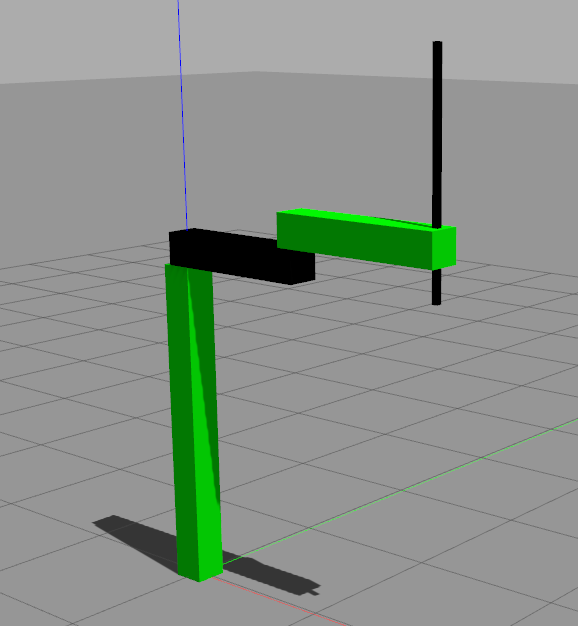
\includegraphics[scale=0.47]{gazebo-final-scara.png}
        \centering
    \end{figure}

    We undertook the following steps to create our SCARA robot.

    \subsubsection{1 --- Modify joint locations}

    In the downloaded package, the RRBot robot has its revolute joints on the `sides' of its links, as shown in the following figure.
    
    \begin{figure}[h]
        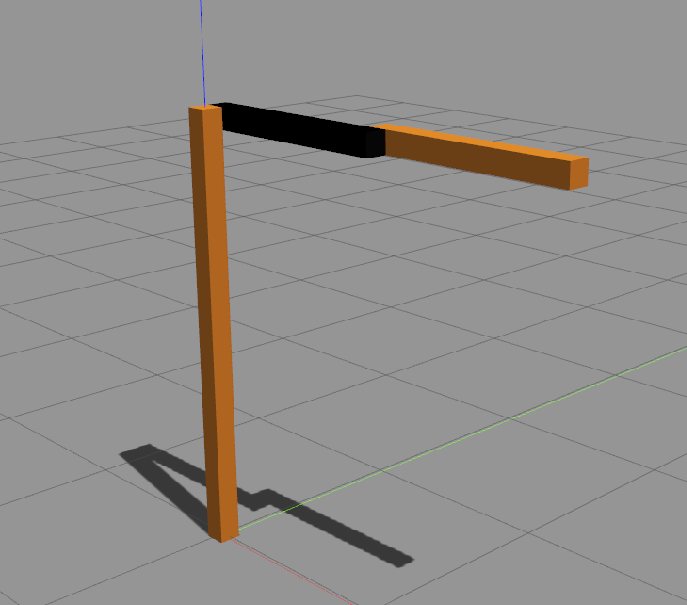
\includegraphics[scale=0.25]{initial-rrbot.png}
        \centering
    \end{figure}

    However, for a standard SCARA robot, we want the revolute joints to sweep angles in the XY plane of the world frame, not in the XZ plane.
    
    Hence, we edited the \lstinline{<joint>} element blocks in the URDF file rrbot\_description.urdf.xacro. For the first joint, we made the following
    change.

    \lstinputlisting[language=XML, firstline=51,lastline=59]{../ros2-code/src/rrbot_simulation_files/rrbot_description/urdf/rrbot_description.urdf.xacro}
    \vspace{0.15in}

    In the above code snippet, we changed the type attribute of the joint element from continuous to revolute. We also added the limit sub-element, and
    modified the origin and axis sub-elements. We made similar changes for the second joint, for which the code snippet is shown below.

    \lstinputlisting[language=XML, firstline=87,lastline=95]{../ros2-code/src/rrbot_simulation_files/rrbot_description/urdf/rrbot_description.urdf.xacro}
    \vspace{0.15in}

    As a result, our robot now looked like the following image.

    \begin{figure}[h]
        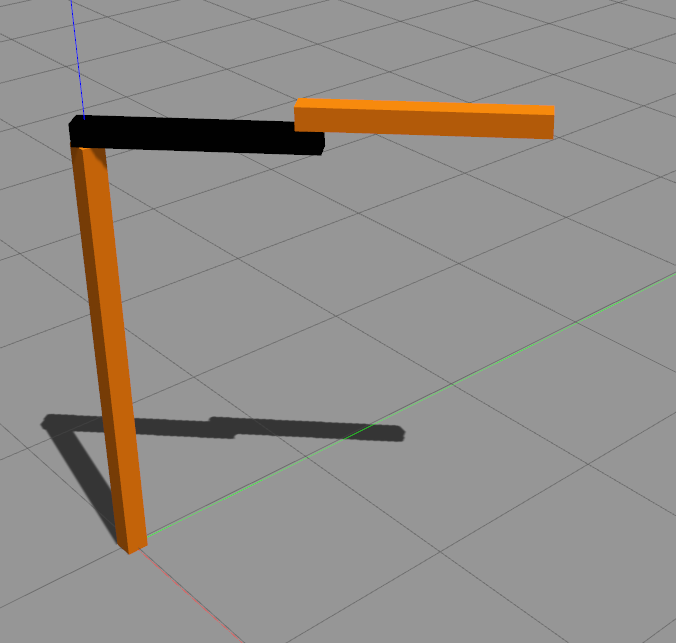
\includegraphics[scale=0.25]{top-joints-rrbot.png}
        \centering
    \end{figure}

\end{homeworkProblem}

\nobreak\extramarks{Question 2}{}\nobreak{}

\pagebreak

\end{document}